
%Inicio del Preámbulo: Modifícalo bajo tu propio riesgo! Usa los paquetes que requieras para 
%implementar funcionalidades dentro del documento. Se comenta solo lo esencial, puedes buscar los
%paquetes y documentarte de su funcionalidad y puedes eliminarlos también si así lo deseas. 

\documentclass[letterpaper,12pt]{article} %Modifica el tipo de documento y el tamaño de la letra.
\usepackage[utf8]{inputenc} %Formato UTF-8 para caracteres especiales.
\usepackage[shortlabels]{enumitem}
\usepackage[spanish,mexico]{babel} 
\usepackage{amsmath,amssymb,amsfonts,latexsym,cancel}
\usepackage[default]{cantarell} %% Use option "defaultsans" to use cantarell as sans serif only
\usepackage[T1]{fontenc}
\usepackage{hyperref}
\usepackage{wrapfig}
\usepackage[rflt]{floatflt}
\usepackage[pdftex]{graphicx}
\usepackage{fancyhdr} %Paquete para el header y el formato de la portada. No sugiero borrarlo!
\usepackage{float}
\usepackage{longtable,multirow,booktabs}
\usepackage{cite}
\usepackage{wrapfig}
\usepackage[square,numbers]{natbib}
\usepackage{multicol}
\usepackage{caption}
\usepackage[]{sidecap}
\usepackage{adjustbox}
\usepackage{parskip}
\usepackage{enumitem}
\usepackage{tikz}
\usepackage{lipsum}
\usepackage[]{xcolor}
\usepackage{graphicx}
\usepackage{listings}
\definecolor{codegreen}{rgb}{0,0.6,0}
\definecolor{codegray}{rgb}{0.5,0.5,0.5}
\definecolor{codepurple}{rgb}{0.58,0,0.82}
\definecolor{backcolour}{rgb}{0.95,0.95,0.92}
\graphicspath{ {imagenes/} }
\lstdefinestyle{mystyle}{
    backgroundcolor=\color{backcolour},   
    commentstyle=\color{codegreen},
    keywordstyle=\color{magenta},
    numberstyle=\tiny\color{codegray},
    stringstyle=\color{codepurple},
    basicstyle=\ttfamily\footnotesize,
    breakatwhitespace=false,         
    breaklines=true,                 
    captionpos=b,                    
    keepspaces=true,                 
    numbers=left,                    
    numbersep=5pt,                  
    showspaces=false,                
    showstringspaces=false,
    showtabs=false,                  
    tabsize=2
}

\lstset{style=mystyle}
%Fin de Préambulo


%Inicio formato de Página. Puedes establecer medidas de la página y modificar el header.

\textheight = 21cm %Medidas de la  página
\textwidth = 18cm  %Medidas de la página
\topmargin = -1cm  %Medidas de la página    
\oddsidemargin = -0.8cm %Medidas de la página
\pagestyle{fancy} %Diseño de la página


\fancyhf{}
\lhead{Facultad de Ingeniería}%%LeftHead
\chead{
\includegraphics[width=1cm, height=1cm]{Imágenes/UNAM.png}}%%CenterHead
%\lfoot{USM}
\rhead{GNU/Linux}%%RightHead

\setlength{\columnsep}{4mm}%Comandos para el formato de la página.
%\setlength{\parindent}{4em}%Sangría al comenzar un nuevo párrafo.
\setlength{\parindent}{0.5in}
%\setlength{\parindent}{4em}%Sangría al comenzar un nuevo párrafo.
\setlength{\parskip}{1em}%Distancia entre párrafos.
\renewcommand{\baselinestretch}{1.5}% Espacio entre línea y línea o interlineado.
\setlength{\headheight}{33pt}
\fancyfoot[CE,CO]{\thepage} %Logo de LaTeX y pie de página.

%Fin formato de Página

%Aquí inicia el documento. Date como magnate
\begin{document}
\lstset{language=bash} 
    %LaTeX te hace el índice automáticamente conforme añades secciones en tu documento.
    %Entorno para portadas

%---------------README----------------->
%USE \include{Portada} %for import front page from main.tex
%USE \usepackage{amsmath} en el preambulo del main
%<<<<<<<<<<<<<<<<<<<<<<<<<<<<<<<<<<<<<<<<<<<

\begin{titlepage}

%--------------- COMANDO LINEA----------------->
\newcommand{\linea}{\rule{\linewidth}{0.7mm}}                 
\center
%<<<<<<<<<<<<<<<<<<<<<<<<<<<<<<<<<<<<<<<<<<<

%Add logos

\includegraphics[width=0.9\textwidth]{logos.png}\\[0.02cm]
\vfill

%---------------TÍTULO----------------->
\linea
\vfill
\textbf{\Large GNU/Linux}\\[0.2cm]
\textbf{\Large Proyecto Final en SHELL}\\[0.8cm]
\linea \\
\vfill

%Title of the Research
\textbf{\large Alumnos:}\\
%<<<<<<<<<<<<<<<<<<<<<<<<<<<<<<<<<<<<<<<<<<<

%Team
    \vfill
    \textbf{\large  \textbf{Roldán Montero Hugo Alejandro}}\\
    \textbf{\large  \textbf{Marquez Sanchez Mirna Daniela}}\\
    \vfill
    
%Fecha or Date
    {\large 21 de Abril de 2023}\\
    \newpage
    \end{titlepage}


    \tableofcontents
    \newpage

\section{Introducción}

En este proyecto se aplicarán los conocimientos adquiridos durante el curso de GNU/Linux, mediante la implementación de un emulador de una terminal, esta terminal cuenta con diferentes características establecidas, haciendo uso del lenguaje "bash" en Shell Script, se tocarán temas como la estructura de linux, implementación de código, sentencias condicionales (if, case, while, for) y comandos esenciales en el uso de linux, junto con sus banderas.

\section{Desarrollo}

Para este proyecto utilizamos bash, en una terminal de Linux, sistema "Unix like" mediante la creación de scripts, se solicitaron en general las siguientes características, mas adelante se desglosará como hicimos cada uno de los scripts, explicados:
\begin{itemize}
    \item Un sistema de acceso
    \item Interacción por línea de comandos
    \item Bloqueo de las señales para salir de la terminal (Ctrl + C / V)
    \item Creación del comando 'ayuda'
    \item Comando "infosis"
    \item Comando "buscar"
    \item Comando que muestre fecha y hora
    \item Comando que muestre los créditos del programador
    \item Comando de juego de gato
    \item Comando de juego de ahorcado
    \item Comando de reproductor MP3
    \end{itemize}

    \begin{itemize}
     \item \textbf{Comando 'MP3':} \\
    Este fue uno de los más laboriosos de utilizar, ya que requeríamos de previamente seleccionar las canciones que queríamos utilizar, para ingresarlas en una carpeta que contuviera las reproducciones, posteriormente se elegirá una canción con "opcion" el cual da la opción al usuario de elegir entre distintas canciones que hemos elegido para él/ella. 
    Incluso al seleccionar algunas canciones que contengan información completa, nos muestra el año, artista, año. 
    Lo que cumple con la función completa de cómo se ve un mp3 al que nosotros estamos acostumbrados a utilizar. 
\begin{lstlisting}
    #!/bin/bash
trap  ''  2  20

prueba=/etc/sgml/pi

if [ -d "$prueba" ]
	then
	sudo mkdir /etc/sgml/pi2
	clear
else
	clear
	echo "Porfavor ingresa la contrasena para reproducir musica" 
	sudo apt -y  install mpg123
 	clear	
 	sudo mkdir /etc/sgml/pi
fi	
	
clear
bandera2=0

while [ $bandera2 -ne 1 ]
do

	echo -e "\e[36mUbicacion de la carpeta puede ser ruta absoluta "
	echo -e "o relativa antes de un epacio porfavor colocar '\' \e[0m"
	read -e ubiact

	opcion=0
	band=1

	while [ $opcion -ne 2 ]
	do
	    clear

	    echo -e "Te encuentras en \e[1;32m$ubiact\e[0m "
	    echo "Menu del reproductor prebeshell: "
	    echo "Reproduce todas las canciones de la carpeta con '1'"
	    echo "Salir del reproductor prebeshell con '2'"
	    echo "deseas cambiar de carpeta '3' si "
	    echo "Que quieres hacer"
	    read -e opcion

	    if [ $opcion -le 0 -o $opcion -ge 4 ]
	    then
	      echo "Error numero no existe profavor ingrese cualquier tecla para continuar"
	      read -e opcion
	      opcion=0;
	    elif [ $opcion -eq 3 ]
	    then
	     	opcion=2
	    elif [ $opcion -eq 2 ]
	    then
	    	bandera2=1
	    	

	    else
	    	command clear

	    
	    	if [ $opcion -eq 1 ]
	    	then

		        cont=1
		        for archivo in $ubiact/*.mp3; do
		        
		        	canciones[$(($cont-1))]="${archivo##*/}"
		        	cont=$(($cont+1))
		        done

		        if [ $(which mpg123) ]
		        then

			        while [ $band -eq 1 ]
			        do
			        	echo -e "\e[34mEste es el Menu de reproduccion de directorio \e[0m"
			            echo -e "Estas en la carpeta \e[32m$ubiact\e[0m"

			            cont=1
			            for archivo in $ubiact/*.mp3; do
			              echo "$cont. ${archivo##*/}"
			              canciones[$(($cont-1))]="${archivo##*/}"
			              cont=$(($cont+1))
			            done

			            echo -e "\e[32mDime el nombre de la cancion o utiliza los siguiente comandos\e[0m"
			            echo "Reproduce la lista de canciones con  '*'."
			            echo "Salir del menu de reproduccion de la carpeta con !"
			            echo " "
			            read -e opcion

			            if [ "$opcion" = "!" ]
			            then
			              band=0

			            elif [ "$opcion" = "*" ]
			            then
				            command clear
				            echo ""
				            echo ""
				            echo "Para quitar reproduccion presione q"
				            echo -e "\e[32mpresiona h para ver el menu de reproduccion\e[0m"
				            echo ""
				            command mpg123 -q "${ubiact}"/*


			            else
				            echo "${ubiact}"/"${opcion}.mp3"
				            echo "Para quitar reproduccion presione q"
				            echo -e "\e[32mpresiona h para ver el menu de reproduccion\e[0m"
				            echo ""
				            command mpg123 -C "${ubiact}"/"${opcion}.mp3"

				            command clear 
				            echo "Se acabaron las canciones presiona cualquier tecla para continuar"
				            read le
			            fi

			            command clear

			            opcion=0
			        done
		        	band=1
		        fi
		    fi
			
			fi
	done
done

command clear
\end{lstlisting}
\end{itemize}

 \begin{figure}[H]
\caption{Ejemplo de reproducción}
\centering
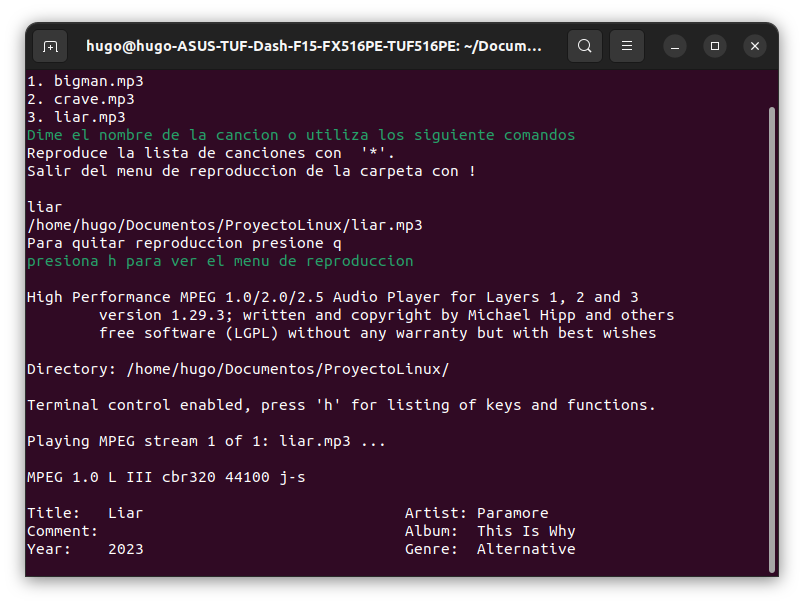
\includegraphics[width=1\textwidth]{Imágenes/LIAR.png}
\end{figure}


\begin{itemize}
     \item \textbf{Comando 'juego de gato':} \\
    Este juego es interactivo para dos personas, a ambos jugadores al inicializar el programa, se le asigna un símbolo diferente, esto lo hacemos con "symbol", utilizamos una lógica de tipo matricial, ya que se seleccionan las columnas y filas para indicar dónde será puesto el símbolo del jugador, de ya contener un símbolo, nos da un mensaje que no se encuentra disponible, o si damos un valor fuera del rango, nuestro programa también lo detecta. 
    De no haber ganador, podemos reiniciar el juego y comenzar otra vez. 
    
\begin{lstlisting}
    #! /bin/bash

iniciarjuego()
{
    echo "====================================================="
    echo "| |              JUEGO DE GATO PADRE              | |"
    echo "| |                      :)                       | |"
    echo "| |                 (2 jugadores)                 | |"
    echo "====================================================="
    echo ""
    echo "Preparando el juego...."
    echo ""
    jugadorgato=1
    tablero=(- - - - - - - - -)
    ganador=1
    echo "*****************************************************"
    echo "| |                                               | |"
    echo "| |          ¡¡¡INICIA EL JUEGO!!!                | |"
    echo "| |                                               | |"
    echo "*****************************************************"
}

imprimirtablero()
{
    echo "Rows\Columns   0   1   2 "
    echo ""
    echo "             -------------"
    echo "    0        | ${tablero[0]} | ${tablero[1]} | ${tablero[2]} |"
    echo "             -------------"
    echo "    1        | ${tablero[3]} | ${tablero[4]} | ${tablero[5]} |"
    echo "             -------------"
    echo "    2        | ${tablero[6]} | ${tablero[7]} | ${tablero[8]} |"
    echo "             -------------"   
}

setInput()
{
   lugares=$(( $1 * 3 + $2 ))
   if [ ${tablero[$lugares]} == "-" ]
   then 
      tablero[$lugares]=$3
      jugadorgato=$((jugadorgato%2+1))
   else
      echo -e "\n--CUIDADO-- ESTE LUGAR YA ESTÁ OCUPADO"
      echo -e "Intenta otra vez!!!!"
   fi
}

checarganador()
{
   simbolos 0 1 2
   simbolos 3 4 5
   simbolos 6 7 8
   simbolos 0 4 8
   simbolos 2 4 6
   simbolos 0 3 6
   simbolos 1 4 7
   simbolos 2 5 8
}

simbolos()
{
   if [ ${tablero[$1]} != "-" ]&&[ ${tablero[$1]} == ${tablero[$2]} ]&&[ ${tablero[$2]} == ${tablero[$3]} ]
   then 
	ganador=0
   fi
}

iniciarjuego
while true
do
	echo ""
	if [ $jugadorgato == 1 ]
  	  then 
  	     symbol=X
  	  else
  	     symbol=O
  	  fi
  	  
	  echo "Jugador $jugadorgato es tu turno: ($symbol)"
          echo ""
	       imprimirtablero
          echo ""
	  echo "#####################################################"
          echo "||                                                 ||"
          echo "||                Inserta la letra :               ||"
          echo "||            A. para jugar Ej: A (fila) (columna) ||"
          echo "||            B. Reset                             ||"
          echo "||            C. Salir                             ||"
          echo "#####################################################"
          echo ""
   
          while true
          do
          printf "Teclea una letra: ";read -r inputCommand a b
          case $inputCommand in
          "A")
          setInput $a $b $symbol
          break
          ;;
          "B")
          iniciarjuego       
          ;;        
          "C")
          exit 0
          break
          ;;
          *)
          echo ""
          echo "Comando no disponible, intenta otra vez"
          ;;
          esac
          
          
            #read -r inputCommand a b
            #if [ $inputCommand == "A" ]
            #then 
 		#setInput $a $b $symbol
                #break
            #elif [ $inputCommand == "reset" ]
            #then 
             #   iniciarjuego
             #   break
            #else
	     #   echo ""
              #  echo "Comando no disponible, intenta otra vez"
	    #fi
          done
   
	  checarganador
	  
          if [ $ganador != 1 ]
	  then
	      jugadorgato=$((jugadorgato%2+1))
	      imprimirtablero
	      echo "=====================================================" 
	      echo "| |                                               | |"
              echo "| |           FIN DE LA PARTIDA               | |"
              echo "| |    jugador $jugadorgato ($symbol) gana     | |"
	      echo "| |                                               | |"
	      echo "====================================================="
	      echo ""
              echo "Escribe la palabra \"reset\" para reinciar el juego" 
     	      read -r inputCommand n
	      while true 
	      do
           	 if [ $inputCommand == "reset" ]
		 then 
                    iniciarjuego
		    break
		 fi   
	      done
	 fi	
done
\end{lstlisting}

 \begin{figure}[H]
\caption{Juego en terminal}
\centering
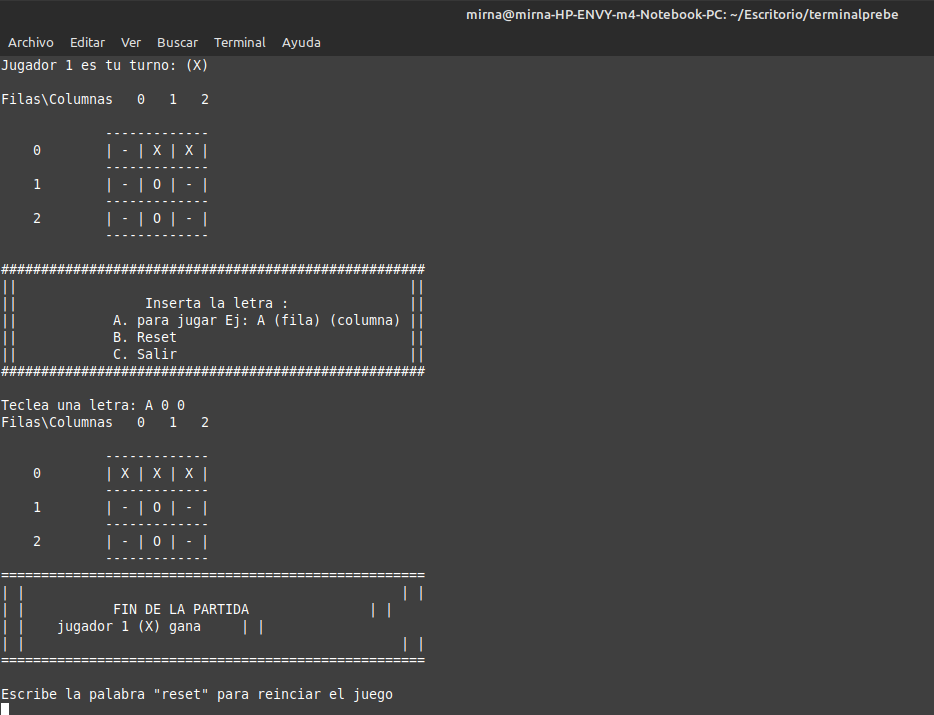
\includegraphics[width=1\textwidth]{Imágenes/capturagato.png}
\end{figure}
\end{itemize}

\begin{itemize}
     \item \textbf{Comando 'juego de ahorcado':} \\
    En este juego utilizamos una metodología muy sencilla, donde cada palabra ingresada por el usuario es repetida con un echo y después de eso es comprobada con la palabra inicial a adivinar. 
    Sigue la estructura de que es para 2 o más jugadores, jugarán 1 vs 1, el jugador ingresa la palabra que desea que el otro jugador adivine, así pues el jugador adivinador tiene 5 intentos de adivinar, de no ser así, hicimos gráficamente un pequeño personaje que irá apareciendo al no ser correcta la palabra, esto con la variable de 'error' que compara letra por letra. Hasta adivinar la palabra, o no; dejamos la adivinanza en manos de nuestro usuario. 
    
\begin{lstlisting}
#!/bin/bash

 '
     _____
    |   \|
    |    |
    |    |
         |
         |
 ________|____
 
 
    _____
    |   \|
    |    |
    0    | ERROR. Esa letra no es correcta
         |
         |
 ________|____
 
    
    _____
    |   \|
    |    |
    0    |
    |    | ERROR 2. Esa letra no es correcta
         |
 ________|____
 
 
    _____
    |   \|
    |    |
    0    |
   /|\    | ERROR 3. Ya tienes tres errores, ya tienes casi la mitad del cuerpo ¡¡CUIDADO!!
         |
 ________|____
 
 
    _____
    |   \|
    |    |
    0    |
   /|\   |
   /     | ERROR 4. Te queda una oprtunidad mas, Tu PUEDES VAMOS, salva a Panchito
 ________|____
 
 
    _____
    |   \|
    |    |
    0    |
   /|\   |
   / \   | ERROR 5. No te tocaba carnal, PERDISTE 
 ________|____
 '
 
 clear
 echo -n "¿QUE PALABRA VAMOS A ADIVINAR?: "
 read word
 echo
# echo "Pulsa enter para continuar..."
# read continuar
 clear
 letra="*"   
 
 fallos=5 
 
 letras=`echo $word | sed "s/[^${letra}]/*"/g` 
 
 sust=$letras
 
 while [ "$sust" != "$word" ]      
 
       do
 #        clear
 	  echo
          echo "LAS LETRAS SON $sust"
          echo
          sed -n "$fallos,$((fallos+7))p" $0
 	  echo 
 	  echo LETRAS INTRODUCIDAS HASTA AHORA: $a
 	  echo 	
 	  echo -n "INTRODUCE UNA LETRA: "
          read letra
 	  a=${a}$letra
 	  palabra=${letra}$palabra   
 			
          echo
          existe=`echo ${word} | grep ${letra}` 
 
               if [ "$existe" = "" ]
                  then
 	             echo "Esa letra no es correcta, la letra - ${letra} - no es parte de la palabra"
 		     error=$((error + 1))
                     if [ $error = 5 ]
                        then
 #	                   clear
 		 	   fallos=$(($fallos+9))
 			   sed -n "$fallos,$((fallos+7))p" $0
 			   echo "Has cometido $error errores, RIP"
                           echo
			   echo	
			   exit
                        else
                           if [ $error = 1 ]
                              then
                                 echo "Has cometido $error errores"
 			         fallos=$(($fallos+9))
                              else
 			         fallos=$(($fallos+9))		
                           fi
                     fi
 
 		  else
                     sust=`echo $word | sed "s/[^${palabra}]/*"/g` 
               fi
 
                  if [ "${sust}" = "${word}" ] 
                     then
                        echo "¡¡¡FELICIDADES!!! HAS DESCUBIERTO LA PALABRA SECRETA QUE ERA: ${word}."
                	echo
 			echo	
                  fi
 
       done
\end{lstlisting}
 \begin{figure}[H]
\caption{Juego en terminal}
\centering
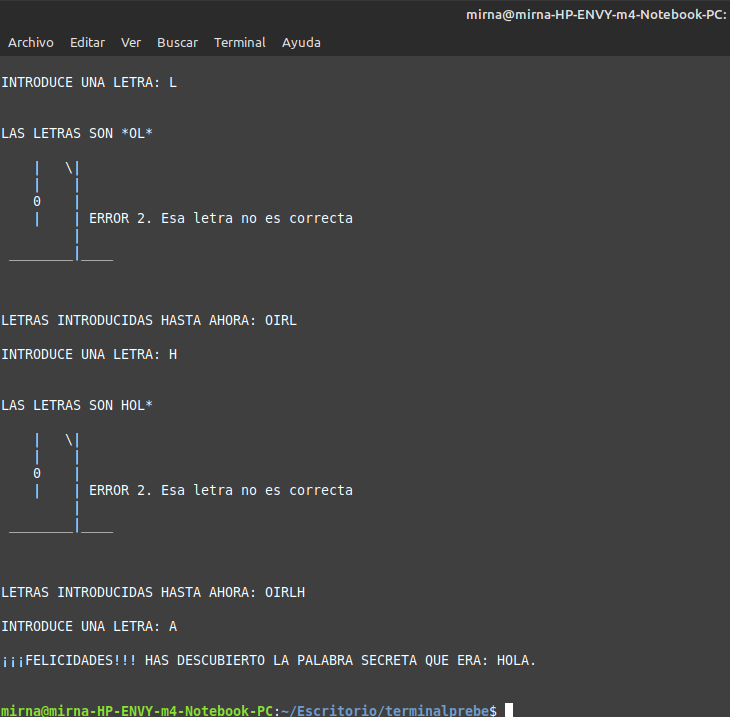
\includegraphics[width=1\textwidth]{Imágenes/terminalahorcado.png}
\end{figure}
\end{itemize}
\clearpage
\begin{itemize}
\item \textbf{Comando 'ayuda'}\\
    Este script, utiliza básicamente los comandos 'echo' cuyo uso es mostrar en pantalla lo deseado, junto con la bandera -e, que nos permitirá interpretar los colores deseados, finalmente, se investigaron los códigos de colores y se aplicaron como se muestra en el código:
\begin{lstlisting}
    #!/bin/bash
rojo="\033[31m"
verde="\033[32m"
azul="\033[34m"
reset_color="\033[0m"

echo -e "${rojo}Los comandos disponibles son:"
echo -e "${azul}ayuda${reset_color}: Proporciona informacion acerca de los comandos disponibles" 
echo -e "${azul}infosis${reset_color}: Proporciona informacion del sistema" 
echo -e "${azul}infodia${reset_color}: Proporciona la fecha y hora actuales"
echo -e "${azul}busca${reset_color}: Busca un archivo en un directorio especifico"
echo -e "${azul}creditos${reset_color}: Muestra los creditos del programa"
echo -e "${azul}MP3${reset_color}: Abrira un reproductor de mp3"
echo -e "${azul}gato${reset_color}: Abrira el juego gato"
echo -e "${azul}ahorcado${reset_color}: Abrira el juego ahorcado"
\end{lstlisting}
    \begin{figure}[H]
\caption{Ejemplo comando ayuda}
\centering
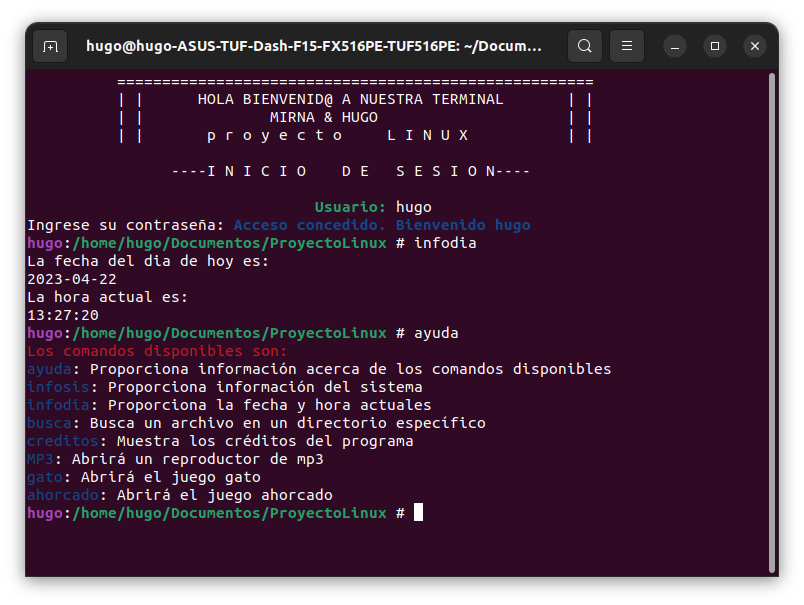
\includegraphics[width=1\textwidth]{Imágenes/ayuda2.png}
\end{figure}
\end{itemize}
\begin{itemize}
     \item \textbf{Comando 'juego de gato':} \\
    Este fue uno de los más laboriosos de utilizar, ya que requeríamos de previamente seleccionar las canciones que queríamos utilizar, para ingresarlas en una carpeta que contuviera las reproducciones, posteriormente se elegirá una canción con "opcion" el cual da la opción al usuario de elegir entre distintas canciones que hemos elegido para él7 ella. 
    Incluso al seleccionar algunas canciones que contengan información completa, nos muestra el año, artista, año. 
    Lo que cumple con la función completa de cómo se ve un mp3 al que nosotros estamos acostumbrados a utilizar. 
    
    \item \textbf{Comando: 'infodia' }:\\ En este caso, se utilizó la carpeta \textbf{/proc/driver/rtc} debido a que en ese archivo, se almacenan los datos de la fecha del sistema, usamos los grep para canalizar la salida solamente a 'rtcdate' y finalmente, otro grep que busque solamente valores numéricos del 0 al 9, seguidos por un guión, la bandera \textbf{-0} indica que este ultimo, deberá ser la salida a mostrar.\\
    En el caso de la hora, se utilizaron las variables de entorno simplemente para mostrar la hora que marca el reloj, quisimos usar dos métodos diferentes para variar el programa.\\
    
    \begin{lstlisting}
    #!/bin/bash
    echo "La fecha del dia de hoy es:"
    cat /proc/driver/rtc |grep 'rtc_date' | grep '[0-9]*-[0-9]*-[0-9]*' -o

echo "La hora actual es: "
printf "%(%H:%M:%S)T\n"
    \end{lstlisting}

\begin{figure}[H]
\caption{Ejemplo comando infodia, que muestra hora y fecha}
\centering
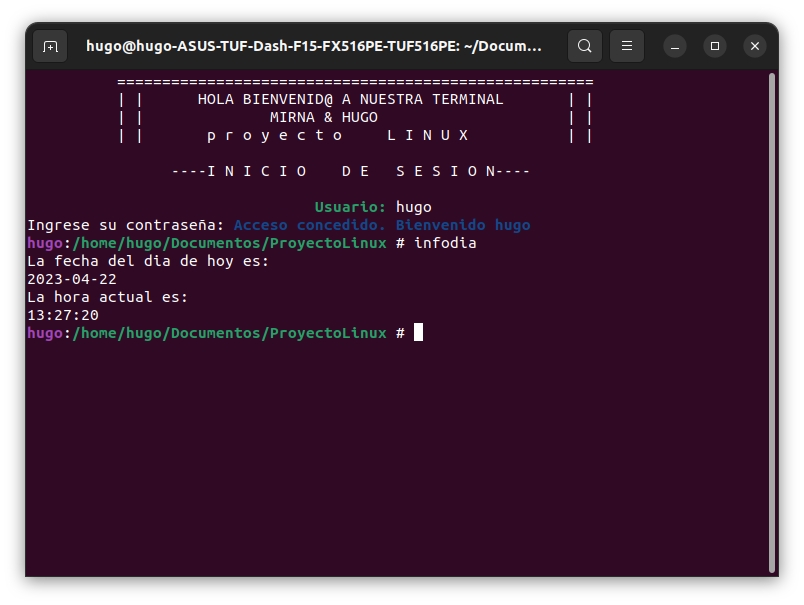
\includegraphics[width=1\textwidth]{Imágenes/infodia2.png}
\end{figure}


     \item \textbf{Comando: Infosis}\\ 
     Para mostrar la información del sistema, primordialmente, se obtuvo de las carpetas de la raíz del sistema, desde etc, hasta proc, de igual forma, se utilizaron cat y grep para canalizar las salidas deseadas según el archivo y se utilizaron colores para contrastar de una mejor manera las salidas.\\
     Para este comando hay muchas alternativas, intenté usar cada una de ellas en el programa, desde cat y grep, hasta utilizar comandos como variables para mostrar la salida.
       \begin{lstlisting}
#!/bin/bash
rojo="\033[31m"
verde="\033[32m"
azul="\033[34m"
amarillo="\033[33m"
sincolor="\033[0m"

echo -e "${rojo}Informacion de la PC y kernel:"
echo ""

echo -e "${rojo}Distribucion y version:${sincolor}"
echo "-----------------------"
cat /etc/os-release | grep -e "^NAME=" -e "^VERSION="

echo -e "${rojo}Informacion de la CPU:${sincolor}"
echo "----------------------"
cat /proc/cpuinfo | grep -m 1 "model name"
echo -e "${rojo}Arquitectura del sistema:${sincolor} $(uname -m)"

echo -e "${rojo}Memoria RAM:${sincolor}"
echo "-------------------------------"
lspci | grep -i --color 'RAM memory:'
echo -e "${amarillo}Memoria total:${sincolor} $(cat /proc/meminfo | grep -i "Memtotal:" | grep '[1-9].*' -o)"
echo -e "${azul}Memoria Libre:${sincolor} $(cat /proc/meminfo | grep -i "Memfree:" | grep '[1-9].*' -o)"
    \end{lstlisting}
\begin{figure}[H]
\caption{Ejemplo comando infosis, que muestra algunas especificaciones del sistema}
\centering
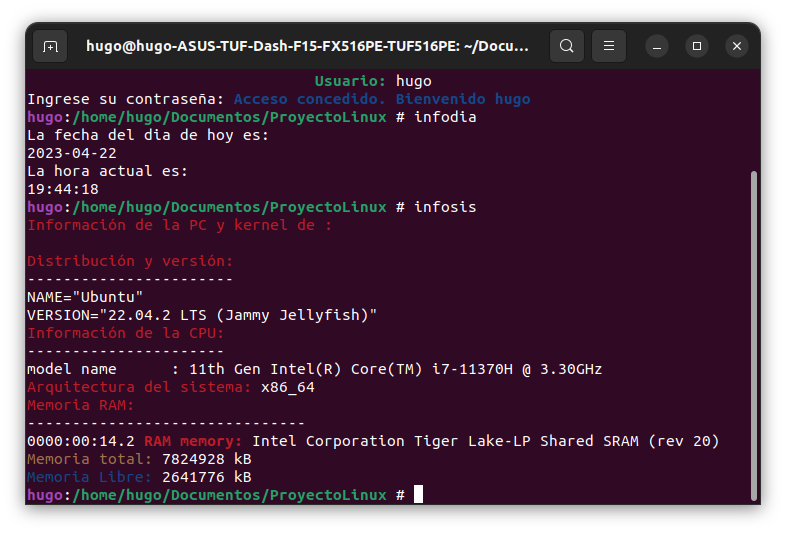
\includegraphics[width=1\textwidth]{Imágenes/infosis.png}
\end{figure}

    
     \item \textbf{Comando: 'creditos'}\\
     En este comando se utilizó solamente el comando echo, imprimiendo cada uno de los datos mostrados en pantalla. En este caso no utilizamos colores para que se vea mas clásico. 
     \begin{lstlisting}
clear
echo -e "\e[97;41m*~~~~~~~~~~~~~~~~~~~~~~~~~~~~~~*\e[0m"
echo -e "\e[97;41m| El desarrollo de esta terminal|\e[0m"
echo -e "\e[97;41m|    fue posible gracias a:    |\e[0m" 
echo -e "\e[97;41m*~~~~~~~~~~~~~~~~~~~~~~~~~~~~~~*\e[0m"
echo -e "\e[97;41m| Marquez Sanchez Mirna Daniela |\e[0m"
echo -e "\e[97;41m|~~~~~~~~~~~~~~~~~~~~~~~~~~~~~~|\e[0m"
echo -e "\e[97;41m| Roldan Montero Hugo Alejandro |\e[0m"
echo -e "\e[97;41m*~~~~~~~~~~~~~~~~~~~~~~~~~~~~~~*\e[0m"
echo -e "\e[97;41m| Gracias por usar nuestra terminal |\e[0m"
echo -e "\e[97;41m|          Hasta pronto! :)  |\e[0m"
echo -e "\e[97;41m*~~~~~~~~~~~~~~~~~~~~~~~~~~~~~~*\e[0m"
     
     \end{lstlisting}
\begin{figure}[H]
\caption{Ejemplo comando creditos}
\centering
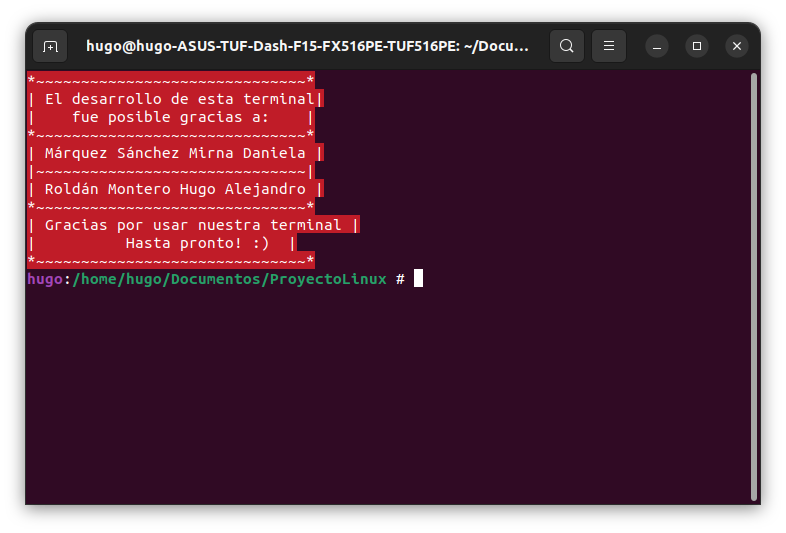
\includegraphics[width=1\textwidth]{Imágenes/creditos.png}
\end{figure}
     \item \textbf{Comando: 'buscar'}\\
     En este comando se utilizó principalmente el comando find.\\
     Comenzamos solicitando al usuario la ruta absoluta y el nombre del archivo que desea encontrar. Para posteriormente abrir dicho directorio.
     Cuando se abre el directorio, guardaremos en la variable 'resultado' el nombre del archivo encontrado, la sentencia se leería asi: 'encontrar un archivo de nombre 'nombre ingresado por el usuario''.\\
     Finalmente se le da formato a la salida y se usa la sentencia if dependiendo si se encuentra o no el archivo.

     \begin{lstlisting}
      #!/bin/bash
# ==-==-==-==-> Solamente son colores
R='\033[1;31m' # Rojo
G='\033[1;32m' # Verde
Y='\033[1;33m' # Amarillo
B='\033[1;34m' # Azul
M='\033[1;35m' # Mangenta
W='\033[0m' # Blanco
Glig='\e[1;32m' # Verde claro
#Pide los parametros

printf "${Glig}Ingrese la ruta absoluta del archivo${W}:"

read -r directorio

printf "${Glig}Ingrese el nombre del archivo con su extension${W}:"

read -r archivo

cd $directorio

# Realiza la busqueda del archivo en el directorio especificado
resultado=$(find -type f -name "$archivo")

if [ -n "$resultado" ]; then
    printf "Archivo encontrado: $R $resultado ${W} en ${M} $directorio ${W}\n"
else
    printf "Archivo ${R}'$archivo'${W} no encontrado en el directorio ${M}'$directorio'${W}\n"
fi  
     \end{lstlisting}
\begin{figure}[H]
\caption{Ejemplo comando buscar}
\centering
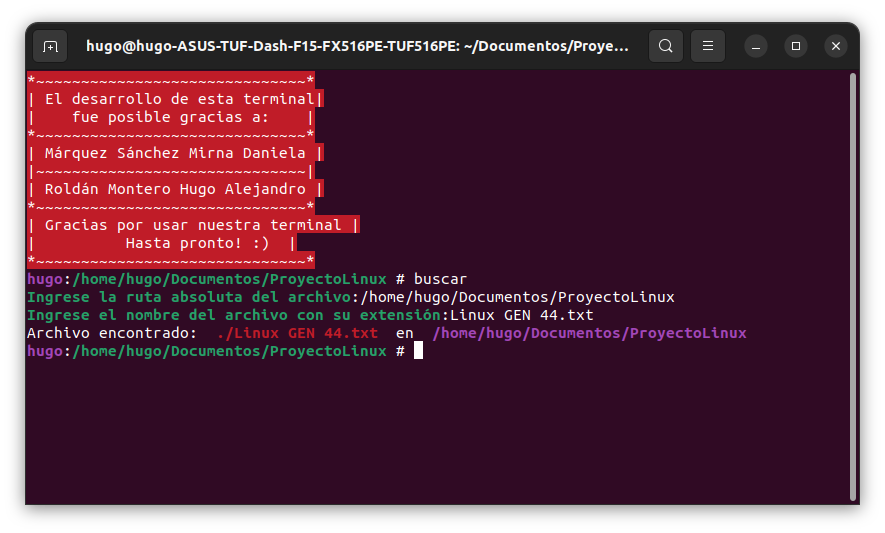
\includegraphics[width=1\textwidth]{Imágenes/buscar.png}
\end{figure}
     \item \textbf{Comando: 'salir'}\\
     En este caso se imprime una salida para despedir al usuario para posteriormente salir de la terminal con la sentencia exit.
    \begin{lstlisting}
    #!/bin/bash
	printf "\t  ===================================================== \n"
	printf "\t  | |               MUCHAS GRACIAS                  | |\n"
	printf "\t  | |               vuelve pronto                   | |\n"
	printf "\t  | |                    :)                         | |\n"
	printf "\n\t\t----C I E R R E    D E   S E S I O N----\n"
        exit 0

    \end{lstlisting}

    \begin{figure}[H]
\caption{Ejemplo comando salir}
\centering
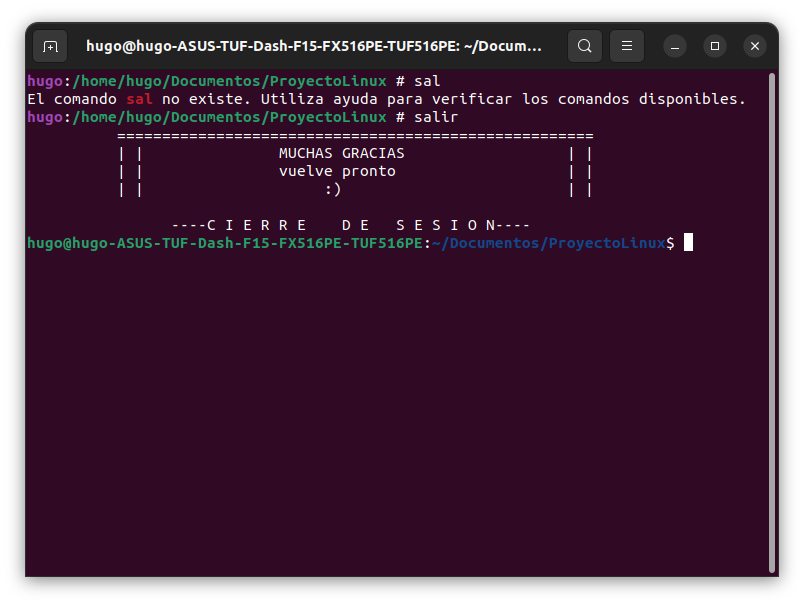
\includegraphics[width=1\textwidth]{Imágenes/SalirN.png}
\end{figure}
\end{itemize}
\newpage

\section{Uso de la terminal}\\
Primero se definirá la función para evitar que se salga de la terminal utilizando los comandos Ctrl + Z/C. \\
En este caso el comando trap, evita que se ejecute cierta sentencia, SIGINT y SIGTSTP, corresponden a los comandos mencionados anteriormente. Si se detecta, llama a la función ignoresignal e imprime en pantalla el mensaje de error.\\
Posteriormente, se implementó el sistema de acceso, se leeran el nombre y contraseña dados por el usuario, para posteriormente corroborar, en la ruta del sistema, si existe el usuario en el sistema y su contraseña es la dada, entonces brindará el acceso, de otra forma, repetira el ciclo para intentar de nuevo.\\
Una vez brindado el acceso, se imprime el usuario proporcionado y la ruta actual del sistema con la variable pwd, que recordando, este comando proporciona al usuario la ubicación actual. posteriormente lee el comando.\\
Para saber como actuar según el comando proporcionado, se implementó un case, en donde cada uno de los casos es un comando de los mencionados en la sección anterior, la acción será ejecutar cada uno de los scripts asociados, en el caso de salir, saldrá del programa. \\
Para el caso default, primero corroborará si el comando existe en el sistema, si lo hace, entonces ejecutará el comando desde el sistema, de otra forma, se mostrará el mensaje de error. \\
\newpage
\begin{lstlisting}
#!/bin/bash

# ==-==-==-==-> Solamente son colores
R='\033[1;31m' # Rojo
G='\033[1;32m' # Verde
Y='\033[1;33m' # Amarillo
B='\033[1;34m' # Azul
M='\033[1;35m' # Mangenta
W='\033[0m' # Blanco
Glig='\e[1;32m' # Verde claro

#Para no salirse

ignore_signal() {
    printf "Se ha detectado la señal $1. No se permite salir. Usa el comando 'salir' para cerrar la terminal.\n"
}

# Configurar la función ctrl + c/z
trap 'ignore_signal SIGINT' SIGINT
trap 'ignore_signal SIGTSTP' SIGTSTP

# Sistema de acceso para los usuarios
# ==-==-==-==-==-==-==-==-==-==-==-==-
clear

printf "\t  ===================================================== \n"
printf "\t  | |      HOLA BIENVENID@ A NUESTRA TERMINAL       | |\n"
printf "\t  | |              MIRNA & HUGO                     | |  \n"
printf "\t  | |       p r o y e c t o     L I N U X           | |\n"
printf "\n\t\t----I N I C I O    D E   S E S I O N----\n"

# ==-==-==-==-> Solicitud de datos (interaccion con el usuario)
# solicitar el nombre de usuario y la contraseña


while true; do
	printf "$G\n\t\t\t\tUsuario: $W"
    read -p "" username
    read -sp "Ingrese su contraseña: " password
    # Verifica si el usuario y la contraseña son válidos en el sistema operativo anfitrión
    if id -u "${username}" >/dev/null 2>&1 && echo "${password}" | su - "${username}" -c 'exit' 2>/dev/null; then
        echo -e "${B}Acceso concedido. Bienvenido ${username}${W}"
        break
    else
        printf "\n\n$R Usuario o contraseña incorrectos. Intente nuevamente.$W\n\n"
    fi
done

while true; do
    # Leer la entrada del usuario
    printf "${M}${username}${W}:${G}$(pwd)${W} # "; read command
    case $command in
    salir)
    exec ./salir.sh
    break
    ;;
    ayuda)
    ./ayuda.sh
    ;;
    infosis)
    ./infosis.sh
    ;;
    infodia)
    ./infodia.sh
    ;;
    MP3)
    ./MP3.sh
    ;;
    buscar)
    ./buscar.sh
    ;;
    creditos)
    ./creditos.sh
    ;;
    gato)
    ./gato.sh
    ;;
    *)
    if command "$command" >/dev/null 2>&1; then
                "$command"
       else 
    printf "El comando $R$command$W no existe. Utiliza ayuda para verificar los comandos disponibles.\n"
    fi
    ;;
    esac
done 
\end{lstlisting}
\begin{figure}[H]
\caption{Ejemplo Terminal corriendo}
\centering
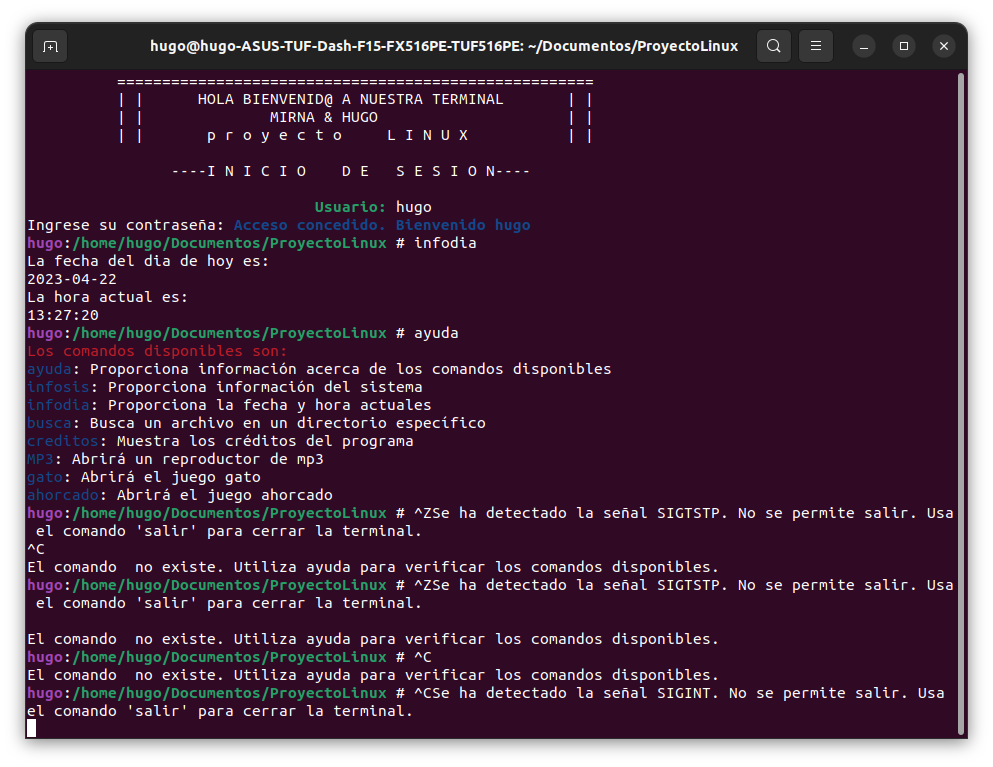
\includegraphics[width=1\textwidth]{Imágenes/Usoterminal.png}
\end{figure}







\clearpage

\section{Conclusion}

\begin{itemize}
    \item \textbf{Mirna:} Fue un proyecto un tanto complicado, ya que había conceptos los cuáles ya teníamos un tanto olvidados e igualmente funcionalidades que habíamos visto de manera superficial en nuestras clases y ahora tendríamos que utilizarlos a su 100 por ciento, era difícil tratar de mejor o modificar algo en nuestra terminal para hacerla diferente, más "adornada" e implementar mejoras, pero como todo programador, mueves 1 cosa y fallan 20, es un proyecto ambicioso en donde tratamos de sacar el mejor provecho, aprender cosas nuevas y juntar todos los conocimientos para llegar a esto, algo tangible, algo grande, algo que es nuestro desde la raíz, por lo que lograrlo es gratificante para nosotros y ver por todo el camino que hemos pasado desde que somos prebes y empezamos a las pocas semanas por este curso y todo lo que hemos recorrido. 
    
    \item \textbf{Hugo:} Este proyecto fue un reto para mí, debido a que varias de las cosas que pedía tenía que investigarlas, ya que si bien, se trataron algunos temas, algunas sentencias o archivos necesarios, era necesario documentarse para saber que archivo guarda específicamente cada cosa para poder imprimirlo en pantalla, si bien, una vez que lo vas empezando, se hace mas ameno, fue un proyecto que disfruté de realizar, ya que reafirmé mis conocimientos en linux, en bash y en latex, además, la satisfacción al ver que tu programa funciona como esperabas es grande. \\
    Finalmente, es un buen ejercicio para reafirmar todos aquellos conocimientos y adquirir otros mas, además de práctica, por lo tanto, me siento satisfecho con el proyecto a entregar. :)

\centering\vspace*{\fill} 
    
\end{itemize}

\end{document}

 %Fin del documento.